\subsection{Model-driven fitting methods}
When acquiring sensor data from physical objects it is often difficult or even impossible to analytically describe the resulting value, as there are numerous environmental factors influencing the signal and the properties of the object might not be clearly determined. Considering the human body, there is a mostly unconstrained number of sizes, shapes and biological properties that influence the response to an electric field. Thus, in order to fit sensor outputs to the potential object configurations, simplified models can be used that resemble the actual physical effects and can be described analytically. Regarding capacitance of the human body relative to a single sensor, a common abstraction is a sphere having a diameter close to the height of an average human \cite{seaver1997human}. Models based on a single geometric objects are considered single-body, while connected geometric objects that comprise a single model can be called multi-body. Smith used a model of multiple spheres to approximate arm position and rotation above an array of capacitive proximity sensors \cite{smith1998electric}. Another possibility is adapting the models to a derived physical effect. Harada et al. are using the projected pressure distribution of a virtual skeleton and body model on a flat surface to create a pressure distribution that can be compared to the actual pressure effect generated by an actual human body resting on a set of sensors \cite{harada2000human}. In this section I will describe two novel methods to fit abstracted models of the human body to sensor readings acquired from smart furniture systems. The first method uses a cylindrical human body model to match the posture of one or two bodies on a bed, the second method uses a multi-body skeleton that is fitted to sensor readings determining posture on a chair.
\subsubsection{Single-body models}
\begin{minipage}{\linewidth}
\centering
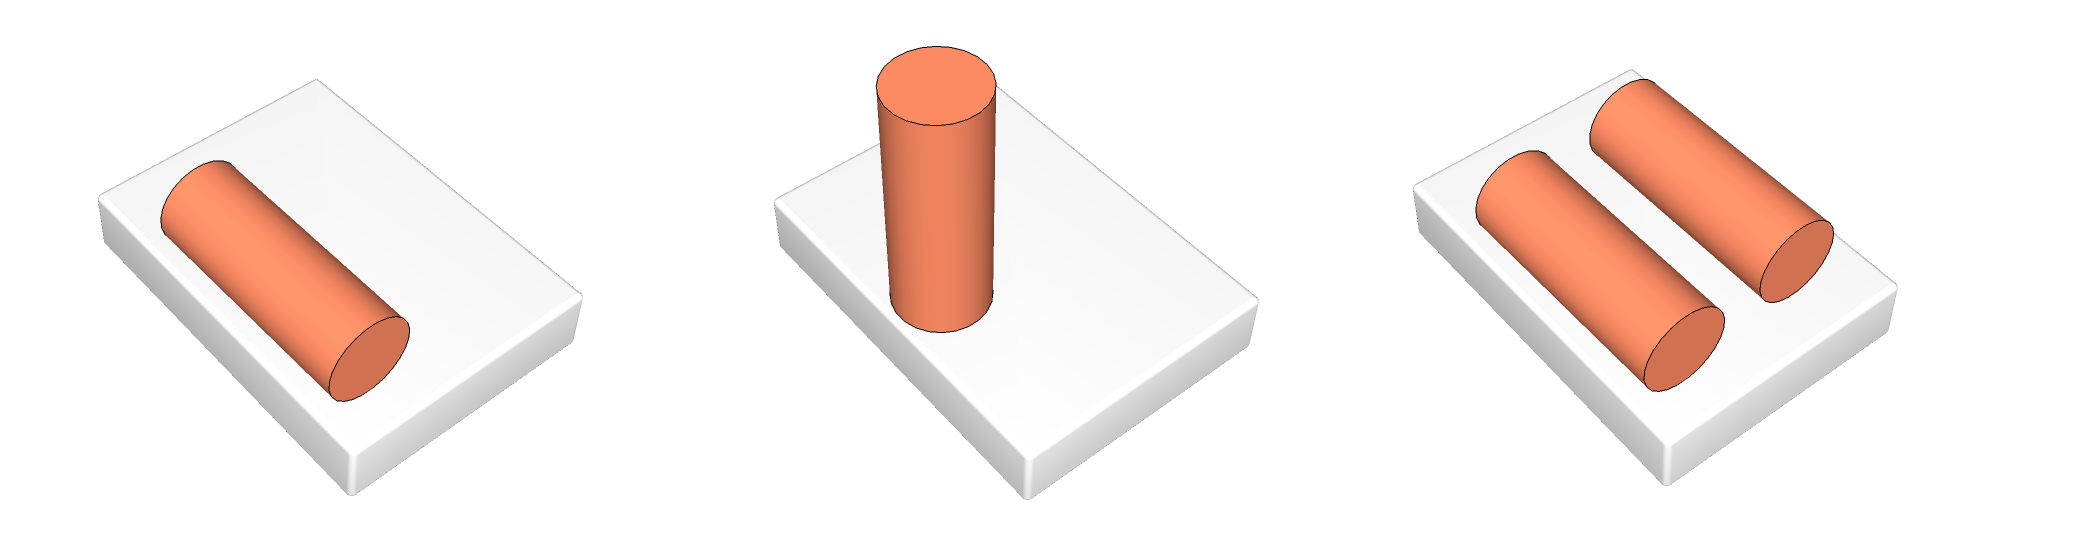
\includegraphics[width=0.8\textwidth]{images/prot_model_bed}
\captionof{figure}{Cylindrical human body model and various poses on mattress}
\label{fig:prot_model_bed}
\end{minipage}	

To identify occupation and positioning we use a very simple model for estimating the effect of a human body on the sensor values. As mentioned earlier the sensors act on both presence and pressure applied. We model the human body as an approximately cylinder shaped object that is on the mattress either lying or sitting, either one or two objects, a few potential poses shown in Figure \ref{fig:prot_model_bed}. We assume that the sensors are analyzing the pressure distribution on the mattress, a sitting person will cause a high pressure on a small region, a lying person a moderate pressure on a larger region. Determining the position and orientation of this cylinder from a limited amount of sensor readings can be postulated as an inverse problem. If we assume a constant density of the cylinder the idealized pressure distribution is uniform as shown in Figure \ref{fig:prot_model_pressure}.

\begin{minipage}{\linewidth}
\centering
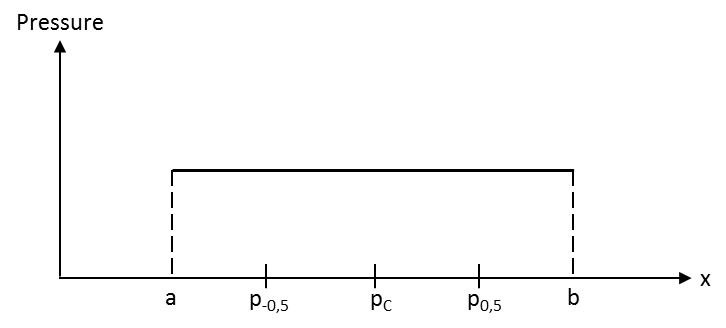
\includegraphics[width=0.6\textwidth]{images/prot_model_pressure}
\captionof{figure}{Pressure distribution of a uniform cylinder}
\label{fig:prot_model_pressure}
\end{minipage}

We further simplify the system by using two distinct values of the pressure distribution. $p_c$ is the center of pressure, $p_{-0.5}$ and $p_{0.5}$ the points enclosing half of the pressure distribution. Using the calculations of a regular uniform, continuous distribution we get the following equations:

\begin{align}
p_c&=\frac{a+b}{2} & \sigma&=\sqrt{\frac{(b-a)^2}{12}}
\end{align}
\begin{align}
p_{-0.5}&=p_c-\sigma &	p_{0.5}&=p_C+\sigma
\end{align}

The raw data from the sensor is considered as random, uniform sampling, a discretization of the continuous distribution. We calculate the center of pressure and the standard deviation of using the geometric meta-information, the position of the sensor $\overrightarrow{x}$.
\begin{equation}
p_c=\frac{\sum_{i=1}^n{v_i\overrightarrow{x}}}{\sum_{i=1}^n{v_i\overrightarrow{x}}}
\end{equation}
\begin{equation}
\sigma=\sqrt{\frac{1}{n}(\sum_{i=1}^n{\overrightarrow{x}^2}-\frac{1}{n}(\sum_{i=1}^n{\overrightarrow{x}})^2}
\end{equation}

Using this model we have determined a set of potential poses that cover the most common situations. We distinguish between potential poses for one and two occupants. One person may sit at a certain location or lie on the bed in various angles. It is assumed that the head is always at the upper part of the bed. Two persons may either both sit, both lie down, or one is sitting and one lying. 
The limitations of this model concerning the actual system are the non-uniform pressure propagation throughout the mattress, as well as the non-linear sensor response on different pressure levels. Therefor we do not expect the deviations to strictly adhere to the theoretical model but instead use configurable thresholds that allow for increased robustness in exchange for precision.

\begin{minipage}{\linewidth}
\centering
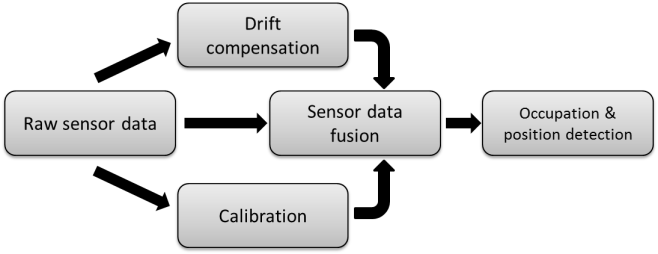
\includegraphics[width=0.7\textwidth]{images/smartbed_proc}
\captionof{figure}{Data processing components \cite{braun2012context}}
\label{fig:smartbed_proc}
\end{minipage}

The different components of the Smart Bed data processing are shown in Figure \ref{fig:smartbed_proc}. Raw sensor data is distributed to three different modules, the calibration which is determining the initial parameters for the sensor data fusion, the drift compensation that alters those parameters according to long term trends and finally the sensor data fusion module that processes the data and does feed it to the occupation \& position detection. Calibration and drift compensation follow the previously presented model \cite{braun2012context}. 

\begin{minipage}{\linewidth}
\centering
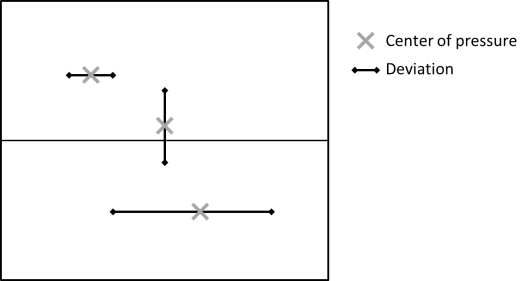
\includegraphics[width=0.7\textwidth]{images/smartbed_cog}
\captionof{figure}{Calculating centers of pressures and deviation \cite{braun2012context}}
\label{fig:smartbed_cog}
\end{minipage}

Occupation and position detection is performed by dividing the two person bed into left and right and individually calculating for each side the total sensor values, assumed center of pressure using weighted average and the standard deviation (Figure \ref{fig:smartbed_cog}). The same calculation is done between the two sides to distinguish where is activity or if one person is lying diagonally.
Using these six intermediate values we can now map various poses. If all activity is on one side and the horizontal deviation is low, we can assume that one person is sitting. We can additionally use the intermediate values to calculate more information, e.g. the exact location a person is sitting at. 
The data processing for the sleep phase recognition is based on detecting the sensor data variations in order to analyze movement. Discriminating between sleep phases using movement is a common approach that has been used in the past \cite{salmi86}. Using a sparse set of sensors it is possible to detect movement by comparing subsequent sensor readings and associate it to different sleep phases using different activity profiles. The system is based on the same prototype as the posture recognition system \cite{Djakow2013movibed}.
\subsubsection{Multi-body models}
\begin{minipage}{\linewidth}
\centering
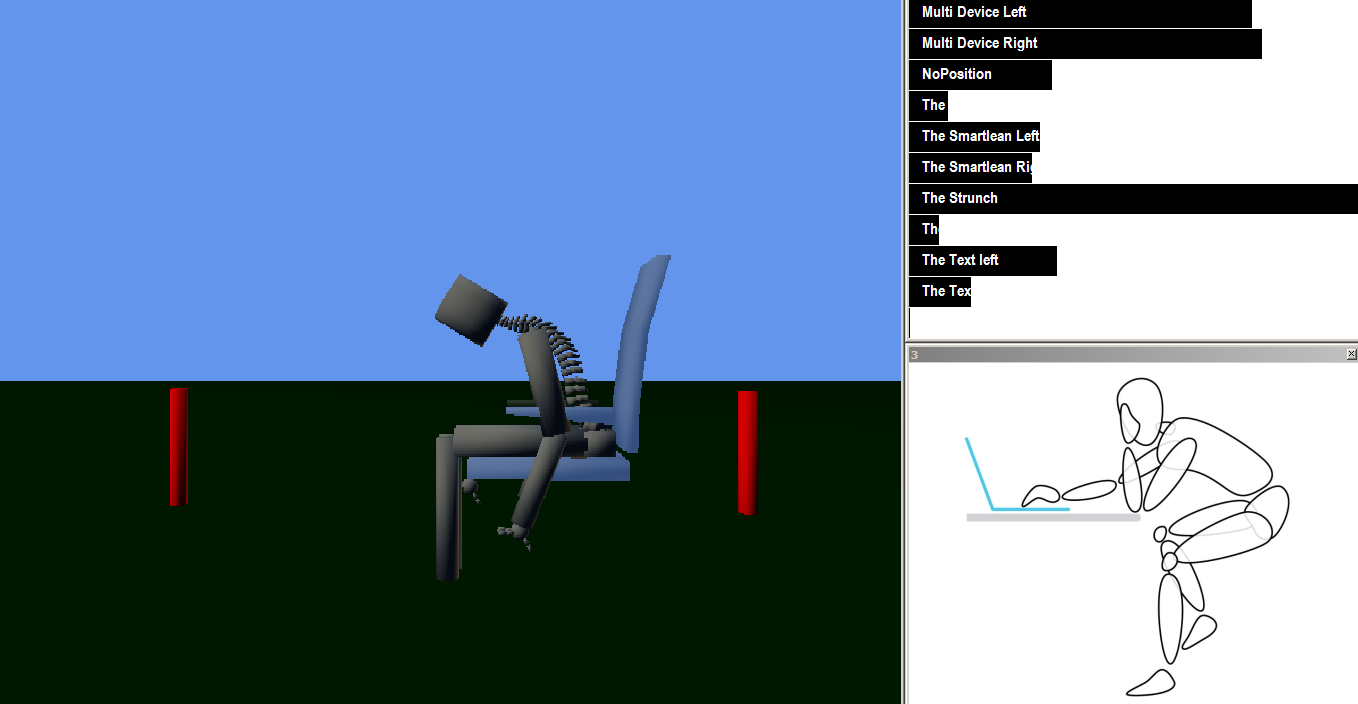
\includegraphics[width=0.7\textwidth]{images/smartchair_software}
\captionof{figure}{Screenshot of the Capacitive Chair application showing the fitted 3D model on the left, posture detection on the upper right and the recognized posture on the lower right}
\label{fig:smartchair_software}
\end{minipage}

In Figure \ref{fig:smartchair_software} we can see a screenshot of the Capacitive Chair debug application. On the left side we see a 3D model that is fitted to a chair model according to the current sensor values, in the middle the results of the machine learning module and the recognized posture and on the right side the currently running breathing rate detection as both Fourier analysis and signal deviation analysis.
All processing methods work on filtered and normalized sensor data. The difference in shape, material and size of the electrodes necessitates slight adaptations to noise filtering and data processing. As an example only the conductive thread backrest electrode is used in the breathing rate detection. 
The 3D model is using a simplified human joint model comprised of 13 connected components. Based on the current sensor readings, single parts or groups of components are fitted to the virtual chair. The process is a mix of posture mapping as found in the smart bed and modification of the dynamic links between the single components \cite{Braun2013ChairAid}.

\begin{minipage}{\linewidth}
\centering
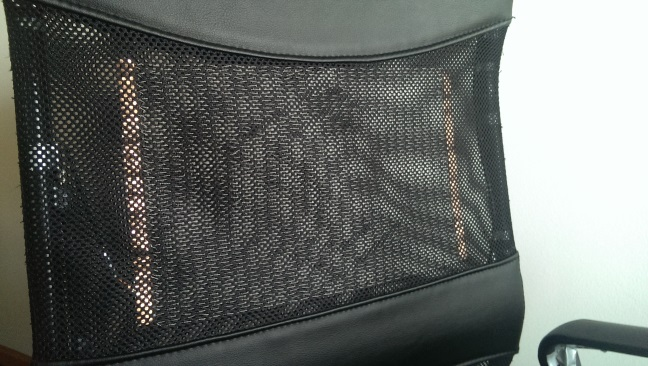
\includegraphics[width=0.7\textwidth]{images/smartchair_thread}
\captionof{figure}{Screenshot of the Capacitive Chair application showing the fitted 3D model on the left, posture detection on the upper right and the recognized posture on the lower right}
\label{fig:smartchair_thread}
\end{minipage}
We use a simple RBF neural network and training data collected by two different persons to match the input from eight sensors to nine potential output postures that are associated to different working situations. An early observation is that certain postures are difficult to distinguish given the limited number of sensors and the similarity of the postures on the rigid chair. Either a higher number of sensors or a more versatile chair could be used that allows gathering additional information required to distinguish the different poses more reliably. 

The breathing rate detection is operating on a single electrode that is integrated into a mesh on the backrest using conductive thread. The setup is shown in Figure \ref{fig:smartchair_thread}. Consequently the surface of the electrode is large and able to pick up the chest movement. Two different methods of data processing are used and fused to get the final breathing rate. Using a fast Fourier transformation the signal is transformed into the frequency space. We are looking for significant signal portions in frequency areas that can be associated to breathing, between $0.2Hz$ and $10Hz$. The second method is to look for zero-crossings of the sensor signal through an adaptive baseline. If a person is breathing in the sensor value will decrease resulting in the signal dropping below the long-term average, and rise above when the person is breathing out. Accordingly the breathing rate can be calculated by counting the zero-crossings.